\section{Teori Resonance Raman dan Formalisme Kramers--Heisenberg--Dirac}
\label{sec:resonance_raman}

\subsection{Kondisi Resonansi dan Interaksi Radiasi-Materi}
Pada spektroskopi Raman konvensional (non-resonansi), energi foton laser eksitasi $\hbar\omega_0$ berada jauh di bawah energi transisi elektronik nyata pertama molekul ($E_e - E_g$). Transisi berlangsung melalui keadaan antara yang bersifat virtual (\textit{virtual intermediate state}) dengan waktu hidup yang sangat singkat ($\tau \sim 10^{-15}\text{ s}$), sebagaimana digambarkan pada Gambar \ref{fig:energy_levels}. Akibatnya, penampang lintang hamburan Raman non-resonansi sangat kecil, berkisar antara $10^{-30}$ hingga $10^{-28}\text{ cm}^2/\text{molekul}$, atau sekitar $10^{10} - 10^{12}$ kali lebih lemah dibandingkan penampang lintang serapan optik fluoresensi.

Sebaliknya, fenomena \textit{Resonance Raman Scattering} (RRS) terjadi apabila energi foton laser eksitasi diatur mendekati atau berimpit tepat dengan energi transisi elektronik molekular atau celah pita optik material:
\begin{equation}
\hbar\omega_0 \approx E_n - E_i,
\label{eq:kondisi_resonansi}
\end{equation}
dengan $|i\rangle$ adalah keadaan awal dan $|n\rangle$ adalah keadaan elektronik tereksitasi nyata. Kondisi resonansi ini menghasilkan penguatan (\textit{enhancement}) intensitas hamburan inelastik hingga mencapai faktor $10^3$ hingga $10^6$ kali lipat. Penguatan selektif ini memungkinkan deteksi sinyal Raman dari lapisan atomik tunggal grafena dan nanotube karbon terisolasi, bahkan pada konsentrasi yang sangat rendah.

\begin{figure}[htbp]
\centering
\resizebox{0.82\textwidth}{!}{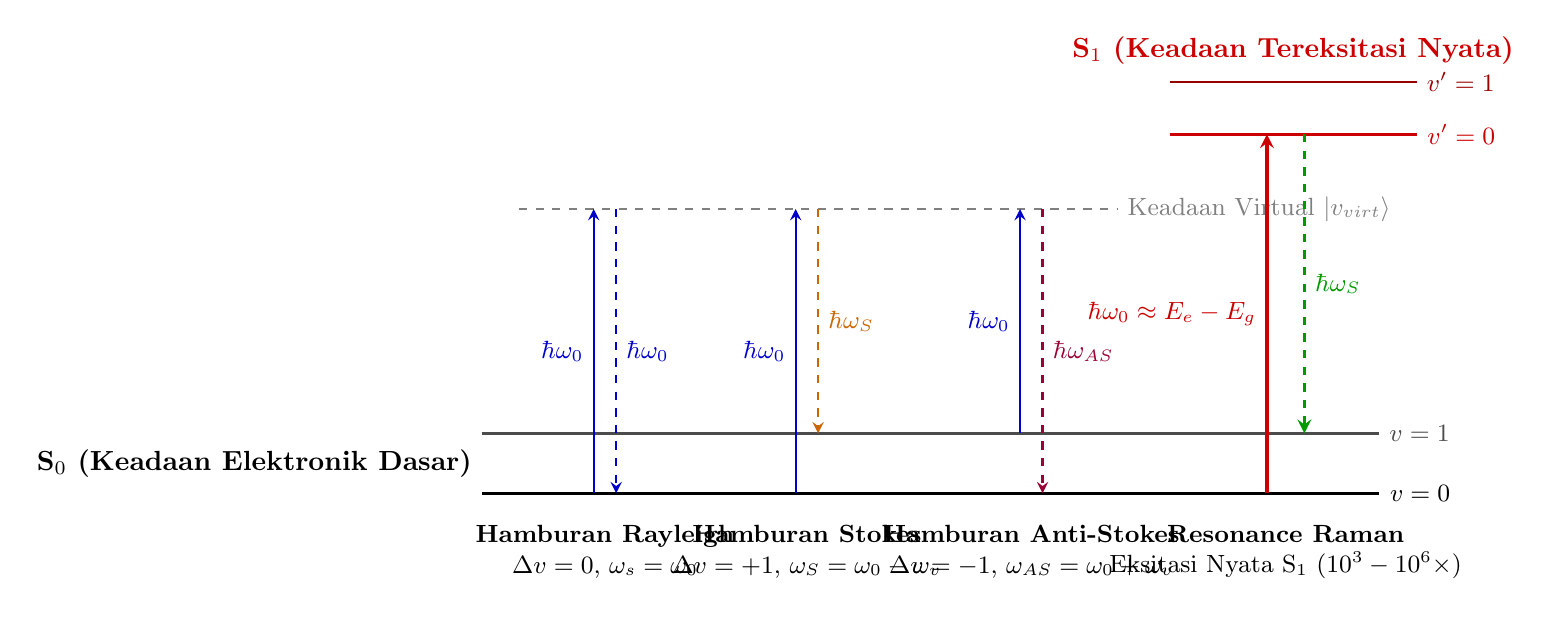
\begin{tikzpicture}[scale=0.95, >=stealth, font=\small]
    % Ground Electronic State S0
    \draw[very thick, black] (0, 0) -- (12, 0) node[right] {$v=0$};
    \draw[thick, black!70] (0, 0.8) -- (12, 0.8) node[right] {$v=1$};
    \node[left, font=\bfseries] at (0, 0.4) {S$_0$ (Keadaan Elektronik Dasar)};
    
    % Virtual States (Dashed)
    \draw[dashed, thick, gray] (0.5, 3.8) -- (8.5, 3.8) node[right] {Keadaan Virtual $|v_{\text{virt}}\rangle$};
    
    % Real Excited Electronic State S1
    \draw[very thick, red!80!black] (9.2, 4.8) -- (12.5, 4.8) node[right] {$v'=0$};
    \draw[thick, red!60!black] (9.2, 5.5) -- (12.5, 5.5) node[right] {$v'=1$};
    \node[above, red!80!black, font=\bfseries] at (10.85, 5.6) {S$_1$ (Keadaan Tereksitasi Nyata)};
    
    % 1. Rayleigh Scattering
    \draw[->, thick, blue!80!black] (1.5, 0) -- (1.5, 3.8) node[midway, left] {$\hbar\omega_0$};
    \draw[->, thick, dashed, blue!80!black] (1.8, 3.8) -- (1.8, 0) node[midway, right] {$\hbar\omega_0$};
    \node[below, align=center] at (1.65, -0.3) {\textbf{Hamburan Rayleigh}\\$\Delta v = 0$, $\omega_s = \omega_0$};
    
    % 2. Stokes Raman
    \draw[->, thick, blue!80!black] (4.2, 0) -- (4.2, 3.8) node[midway, left] {$\hbar\omega_0$};
    \draw[->, thick, dashed, orange!80!black] (4.5, 3.8) -- (4.5, 0.8) node[midway, right] {$\hbar\omega_S$};
    \node[below, align=center] at (4.35, -0.3) {\textbf{Hamburan Stokes}\\$\Delta v = +1$, $\omega_S = \omega_0 - \omega_v$};
    
    % 3. Anti-Stokes Raman
    \draw[->, thick, blue!80!black] (7.2, 0.8) -- (7.2, 3.8) node[midway, left] {$\hbar\omega_0$};
    \draw[->, thick, dashed, purple!80!black] (7.5, 3.8) -- (7.5, 0) node[midway, right] {$\hbar\omega_{AS}$};
    \node[below, align=center] at (7.35, -0.3) {\textbf{Hamburan Anti-Stokes}\\$\Delta v = -1$, $\omega_{AS} = \omega_0 + \omega_v$};
    
    % 4. Resonance Raman
    \draw[->, very thick, red!80!black] (10.5, 0) -- (10.5, 4.8) node[midway, left] {$\hbar\omega_0 \approx E_e - E_g$};
    \draw[->, very thick, dashed, green!60!black] (11.0, 4.8) -- (11.0, 0.8) node[midway, right] {$\hbar\omega_S$};
    \node[below, align=center] at (10.75, -0.3) {\textbf{Resonance Raman}\\Eksitasi Nyata S$_1$ ($10^3 - 10^6\times$)};
\end{tikzpicture}
}
\caption{Diagram tingkat energi yang membandingkan transisi hamburan elastik Rayleigh, hamburan Raman non-resonansi (Stokes dan anti-Stokes via keadaan virtual), dan hamburan \textit{Resonance Raman} (eksitasi nyata keadaan elektronik $S_1$ dengan redaman $\Gamma_n$).}
\label{fig:energy_levels}
\end{figure}

\subsection{Formalisme Kramers--Heisenberg--Dirac (KHD)}
Deskripsi kuantum hamburan inelastik foton dua-tahap diturunkan menggunakan teori gangguan bergantung waktu orde kedua (\textit{second-order time-dependent perturbation theory}). Hamiltonian interaksi radiasi-materi dalam pendekatan dipol listrik diberikan oleh:
\begin{equation}
\hat{H}_{\mathrm{int}} = - \hat{\boldsymbol{\mu}} \cdot \mathbf{E}(t),
\label{eq:hamiltonian_interaksi}
\end{equation}
dengan $\hat{\boldsymbol{\mu}} = -e \sum_k \hat{\mathbf{r}}_k$ menyatakan operator momen dipol listrik molekular.

Amplitudo probabilitas hamburan Raman transisional dari keadaan awal $|i\rangle$ menuju keadaan akhir $|f\rangle$ melalui penjumlahan seluruh keadaan antara $|n\rangle$ dirumuskan oleh persamaan dispersi Kramers--Heisenberg--Dirac (KHD) \cite{kramers1925streuung,dirac1927quantum,albrecht1961theory}:
\begin{equation}
(\alpha_{ij})_{fi} = \frac{1}{\hbar} \sum_{n} \left[ 
\frac{\langle f | \hat{\boldsymbol{\mu}} \cdot \mathbf{e}_s | n \rangle \langle n | \hat{\boldsymbol{\mu}} \cdot \mathbf{e}_i | i \rangle}{\omega_{ni} - \omega_0 - i\Gamma_n} + 
\frac{\langle f | \hat{\boldsymbol{\mu}} \cdot \mathbf{e}_i | n \rangle \langle n | \hat{\boldsymbol{\mu}} \cdot \mathbf{e}_s | i \rangle}{\omega_{ni} + \omega_s + i\Gamma_n}
\right],
\label{eq:khd_amplitudo}
\end{equation}
dengan:
\begin{itemize}
    \item $\mathbf{e}_i$ dan $\mathbf{e}_s$ adalah vektor satuan polarisasi foton datang dan foton terhambur.
    \item $\hbar\omega_{ni} = E_n - E_i$ merupakan selisih energi antara keadaan perantara $|n\rangle$ dan keadaan awal $|i\rangle$.
    \item $\omega_0$ dan $\omega_s$ adalah frekuensi sudut foton eksitasi laser dan foton terhambur.
    \item $\Gamma_n$ adalah parameter redaman fenomenologis (\textit{damping factor}) dari keadaan antara $|n\rangle$, yang berbanding terbalik dengan waktu hidup radiative dan non-radiative keadaan tersebut: $\Gamma_n = \hbar / (2\tau_n)$.
\end{itemize}

Suku pertama pada Persamaan \eqref{eq:khd_amplitudo} dinamakan \textit{resonant term}, sedangkan suku kedua disebut \textit{anti-resonant term}. Ketika energi eksitasi laser mendekati energi transisi elektronik nyata ($\omega_0 \to \omega_{ni}$), penyebut suku resonan mendekati nol:
\begin{equation}
\omega_{ni} - \omega_0 \to 0 \implies \left| \frac{1}{\omega_{ni} - \omega_0 - i\Gamma_n} \right|^2 \to \frac{1}{\Gamma_n^2} \gg 1.
\label{eq:resonansi_dominasi}
\end{equation}
Keberadaan faktor redaman $\Gamma_n \neq 0$ mencegah terjadinya divergensi singularitas matematis tak-hingga dan mencerminkan lebar spektral alami keadaan elektronik perantara. Pada kondisi resonansi penuh, suku resonan mendominasi secara mutlak dan suku anti-resonan dapat diabaikan.

\subsection{Mekanisme Penguatan Albrecht: Franck--Condon dan Herzberg--Teller}
Dalam pendekatan Born--Oppenheimer, fungsi gelombang total dipisahkan menjadi perkalian fungsi gelombang elektronik $|e\rangle$ dan fungsi gelombang vibrasi-inti $|v\rangle$: $|i\rangle = |g, v_i\rangle$, $|n\rangle = |e, v_n\rangle$, dan $|f\rangle = |g, v_f\rangle$. Momen dipol transisi elektronik diekspansikan terhadap koordinat normal vibrasi $Q$:
\begin{equation}
\boldsymbol{\mu}_{ge}(Q) = \boldsymbol{\mu}_{ge}^{(0)} + \sum_k \left( \frac{\partial \boldsymbol{\mu}_{ge}}{\partial Q_k} \right)_0 Q_k + \dots
\end{equation}

Substitusi ekspansi ini ke dalam persamaan KHD menghasilkan pembagian amplitudo polarizabilitas Albrecht menjadi dua suku utama: $(\alpha)_{fi} \approx A + B$ \cite{albrecht1961theory}:
\begin{enumerate}
    \item \textbf{Mekanisme Franck--Condon (Suku $A$ Albrecht)}:
    \begin{equation}
    A = \frac{|\boldsymbol{\mu}_{ge}^{(0)}|^2}{\hbar} \sum_{v_n} \frac{\langle v_f | v_n \rangle \langle v_n | v_i \rangle}{\omega_{ev_n, gv_i} - \omega_0 - i\Gamma_{ev_n}}.
    \label{eq:albrecht_a}
    \end{equation}
    Suku $A$ bergantung langsung pada integral tumpang tindih vibrasi (\textit{Franck--Condon overlap integral}) $\langle v_f | v_n \rangle \langle v_n | v_i \rangle$. Mekanisme ini dominan apabila terjadi pergeseran posisi kesetimbangan potensial inti atom ($\Delta Q \neq 0$) antara permukaan energi potensial elektronik tereksitasi dan keadaan dasar. Suku ini secara selektif memperkuat mode vibrasi total simetris ($A_{1g}$ atau $A_1$).
    \item \textbf{Mekanisme Herzberg--Teller (Suku $B$ Albrecht)}:
    \begin{equation}
    B = \frac{\boldsymbol{\mu}_{ge}^{(0)}}{\hbar} \sum_{e' \neq e} \left( \frac{\partial \boldsymbol{\mu}_{ee'}}{\partial Q_k} \right)_0 \sum_{v_n} \left[ \frac{\langle v_f | Q_k | v_n \rangle \langle v_n | v_i \rangle + \langle v_f | v_n \rangle \langle v_n | Q_k | v_i \rangle}{\omega_{ev_n, gv_i} - \omega_0 - i\Gamma_{ev_n}} \right].
    \label{eq:albrecht_b}
    \end{equation}
    Suku $B$ melibatkan kopling vibronik non-adiabatik antara dua keadaan elektronik tereksitasi yang berbeda ($e$ dan $e'$) yang dipicu oleh mode vibrasi normal $Q_k$. Mekanisme Herzberg--Teller memungkinkan terjadinya penguatan resonansi pada mode vibrasi non-total simetris.
\end{enumerate}

\subsection{Resonansi Ganda (\textit{Double Resonance}) pada Nanomaterial Karbon}
Pada material karbon berstruktur pita elektronik unik seperti grafena dan nanotube karbon, fenomena hamburan Raman diperkaya oleh mekanisme \textbf{Resonansi Ganda (\textit{Double Resonance})}, sebagaimana diilustrasikan pada Gambar \ref{fig:double_resonance} \cite{ferrari2006raman,malard2009raman}.

\begin{figure}[htbp]
\centering
\resizebox{0.82\textwidth}{!}{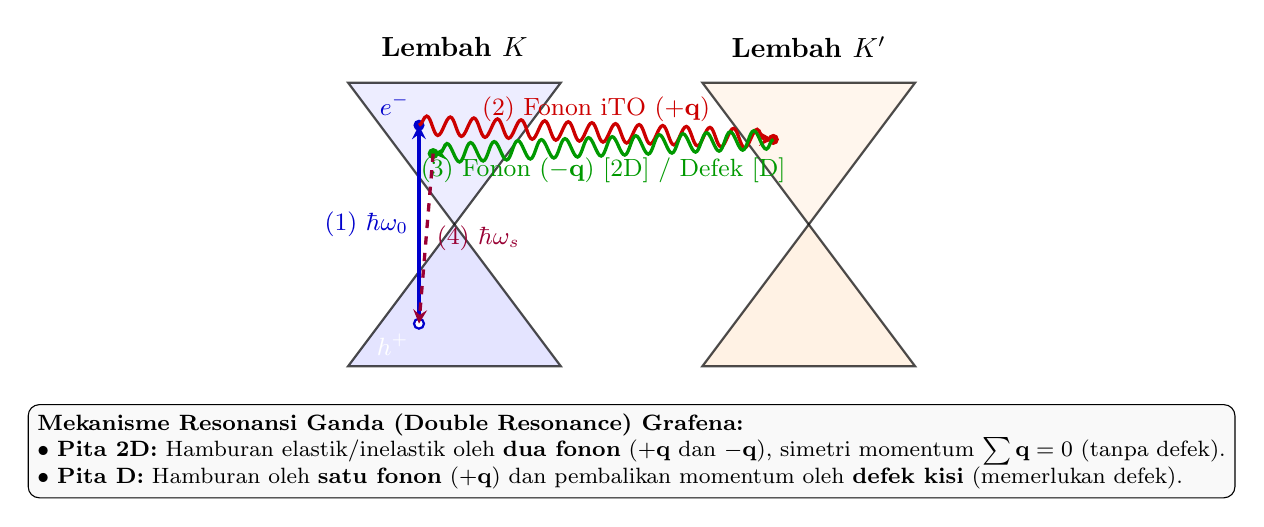
\begin{tikzpicture}[scale=0.9, >=stealth, font=\small]
    % Dirac Cones at K and K'
    \node[font=\bfseries] at (2.5, 4.5) {Lembah $K$};
    \node[font=\bfseries] at (7.5, 4.5) {Lembah $K'$};
    
    % Left Dirac Cone (K)
    \draw[thick, fill=blue!10, opacity=0.7] (2.5, 2.0) -- (1.0, 4.0) -- (4.0, 4.0) -- cycle;
    \draw[thick, fill=blue!15, opacity=0.7] (2.5, 2.0) -- (1.0, 0.0) -- (4.0, 0.0) -- cycle;
    
    % Right Dirac Cone (K')
    \draw[thick, fill=orange!10, opacity=0.7] (7.5, 2.0) -- (6.0, 4.0) -- (9.0, 4.0) -- cycle;
    \draw[thick, fill=orange!15, opacity=0.7] (7.5, 2.0) -- (6.0, 0.0) -- (9.0, 0.0) -- cycle;
    
    % Step 1: Vertical Optical Absorption (e-h pair creation)
    \draw[->, very thick, blue!80!black] (2.0, 0.6) -- (2.0, 3.4) node[midway, left] {(1) $\hbar\omega_0$};
    \filldraw[blue!80!black] (2.0, 3.4) circle (2pt) node[above left] {$e^-$};
    \filldraw[white, draw=blue!80!black, thick] (2.0, 0.6) circle (2pt) node[below left] {$h^+$};
    
    % Step 2: Inelastic Phonon Scattering from K to K' (wavevector q)
    \draw[->, very thick, red!80!black, decorate, decoration={snake, amplitude=1.2mm, segment length=3mm}] 
        (2.0, 3.4) -- (7.0, 3.2) node[midway, above] {(2) Fonon iTO ($+\mathbf{q}$)};
    \filldraw[red!80!black] (7.0, 3.2) circle (2pt);
    
    % Step 3: Second Inelastic Scattering or Defect Backscattering from K' to K
    \draw[->, very thick, green!60!black, decorate, decoration={snake, amplitude=1.2mm, segment length=3mm}] 
        (7.0, 3.2) -- (2.2, 3.0) node[midway, below] {(3) Fonon ($-\mathbf{q}$) [2D] / Defek [D]};
    \filldraw[green!60!black] (2.2, 3.0) circle (2pt);
    
    % Step 4: Radiative e-h Recombination (Emission of Raman Photon)
    \draw[->, very thick, dashed, purple!80!black] (2.2, 3.0) -- (2.0, 0.6) node[midway, right] {(4) $\hbar\omega_s$};
    
    % Bottom Legend
    \node[draw, rounded corners, fill=gray!5, align=left, font=\footnotesize] at (5.0, -1.2) {
        \textbf{Mekanisme Resonansi Ganda (Double Resonance) Grafena:}\\
        $\bullet$ \textbf{Pita 2D:} Hamburan elastik/inelastik oleh \textbf{dua fonon} ($+\mathbf{q}$ dan $-\mathbf{q}$), simetri momentum $\sum \mathbf{q} = 0$ (tanpa defek).\\
        $\bullet$ \textbf{Pita D:} Hamburan oleh \textbf{satu fonon} ($+\mathbf{q}$) dan pembalikan momentum oleh \textbf{defek kisi} (memerlukan defek).
    };
\end{tikzpicture}
}
\caption{Mekanisme hamburan resonansi ganda (\textit{Double Resonance}) pada kerucut Dirac grafena di lembah $K$ dan $K'$ zona Brillouin: pembentukan pasangan elektron-lubang oleh foton datang, hamburan inelastik fonon inter-valley, hamburan balik (oleh fonon kedua pada pita $2D$ atau defek pada pita $D$), dan rekombinasi radiatif memancarkan foton Raman.}
\label{fig:double_resonance}
\end{figure}

Pada grafena, pita konduksi dan valensi bersinggungan secara linier pada titik sudut zona Brillouin heksagonal ($K$ dan $K'$), membentuk kerucut Dirac dengan relasi dispersi tanpa massa: $E(\mathbf{k}) = \pm \hbar v_F |\mathbf{k}|$, dengan kecepatan Fermi $v_F \approx 10^6\text{ m/s}$. Karena tidak adanya celah pita energi, foton eksitasi laser dengan energi sembarang di wilayah optik selalu berada dalam kondisi resonansi optik transisi vertikal langsung antarpita.

Proses resonansi ganda berlangsung dalam empat tahapan mikroskopis:
\begin{enumerate}
    \item Absorpsi foton laser $\hbar\omega_0$ menghasilkan eksitasi vertikal pasangan elektron-lubang nyata pada vektor gelombang $\mathbf{k}$ di sekitar titik $K$.
    \item Elektron terhambur secara inelastik menuju vektor gelombang $\mathbf{k} + \mathbf{q}$ di lembah Dirac tetangga ($K'$) dengan memancarkan fonon in-plane transverse optical (iTO) bervektor gelombang $\mathbf{q}$.
    \item Elektron dihamburkan kembali dari lembah $K'$ menuju lembah asal $K$:
    \begin{itemize}
        \item Pada \textbf{Pita 2D}: proses dihamburkan kembali oleh fonon iTO kedua bervektor gelombang $-\mathbf{q}$. Karena kedua fonon memiliki vektor gelombang berlawanan arah ($\mathbf{q} + (-\mathbf{q}) = 0$), kekekalan momentum kristal terpenuhi secara sempurna tanpa memerlukan keberadaan defek kisi.
        \item Pada \textbf{Pita D}: proses hamburan balik difasilitasi oleh hamburan elastik pada defek kisi struktural atau batas tepi (\textit{edge}). Oleh karena itu, pita $D$ memerlukan defek untuk aktif.
    \end{itemize}
    \item Pasangan elektron-lubang berekombinasi secara radiatif, memancarkan foton hamburan Raman $\hbar\omega_s$.
\end{enumerate}

Konsekuensi mendasar dari proses resonansi ganda ini adalah \textbf{dispersi pergeseran Raman terhadap energi foton laser eksitasi} ($\partial\omega / \partial E_L$). Karena vektor gelombang fonon teresonansi $\mathbf{q}$ terhubung langsung dengan vektor gelombang elektron $k \approx E_L / (2\hbar v_F)$, peningkatan energi laser memperbesar lingkaran resonansi momentum, memicu peningkatan frekuensi fonon teramati sebesar:
\begin{equation}
\frac{\partial \omega_{2D}}{\partial E_L} \approx 100\text{ cm}^{-1}/\text{eV}, \qquad
\frac{\partial \omega_{D}}{\partial E_L} \approx 50\text{ cm}^{-1}/\text{eV}.
\label{eq:dispersi_resonansi_ganda}
\end{equation}

Pada tabung karbon nano (SWCNT), kurvatur silindris memecah kerucut Dirac grafena menjadi deret sub-pita satu dimensi yang memiliki puncak kerapatan keadaan tajam yang dikenal sebagai \textbf{Singularitas van Hove} ($E_{ii}$) \cite{dresselhaus2005raman}. Resonansi Raman pada SWCNT terjadi sangat tajam ketika energi foton laser cocok dengan jarak antar-singularitas van Hove yang bersesuaian, sebagaimana dirangkum dalam diagram Kataura (\textit{Kataura plot}).
